\emph{There are many challenges which arise when trying to carry out a project which must be thoroughly documented and accounted for during the planning stages and subsequent design and implementation. For example, there must be considerations for how the project software will be developed, how the team will be organised, how the tasks will be scheduled and the various tools which will be used throughout the project. This chapter will discuss specific areas of project management such as these, and how the project group overcame the various challenges which arose throughout the duration of the project.}

\section{Project Methodology}

\subsection{Project Summary}
As with any software development project, it is important to first outline the aims of the project, the resources available to achieve these aims, and ensure that the stakeholders in the project have been correctly identified before the project begins. This allows for the project to have a clear view of its objectives and how to reach them. Furthermore, justification for why and how the project should be carried out is necessary to ensure that each group member is satisfied with the direction of the project and their roles within the group. This has been discussed in greater detail in the specification chapter, but will be summarised in this section to outline how the project developed from a management perspective.

The project idea to work with drone sensor networks was unanimously accepted by every group member; with the hardware freely available from the Department, each member was enthusiastic to tackle the various technical challenges which would arise in terms of hardware and software. UAVs and their applications in a sensor network is a subject which is currently a hotbed for research and development, with many different applications. The project deliverable presented an opportunity to experience working on the state-of-the-art in terms of technology and research, with the possibility of a lasting impact on the field.
Using several Parrot AR drones, the objective of the group was to create a simulator for sensor networks which could initialise and control airborne nodes, allowing them to function autonomously, as well as take user input to perform a task. The platform was then to be deployed onto hardware available from the Department, including external computers and extra peripherals.

The project was decided to be made for general use case, but with a focus on making a tool which could be used to perform research and outreach activities. The project supervisor approved the project, and continued to give helpful advice and considerations to assist with the planning stages. After agreeing upon the project, considering the resources and selecting a specific use case to work towards, the following work involved researching current methods and designing a simulation for the network. Once the simulation environment had been completed, communications and physical routing would be incorporated into the design, before finally transferring the platform onto the real drones for physical deployment. Each stage of the project was carefully monitored (as described later in this chapter), and tasks were split evenly between the group members in order to ensure that the project was completed within time constraints. Monitoring also ensured that any potential problems were addressed as they appeared. In the final stages of the project, the project deliverables, including the necessary documentation, were finalised and brought to a conclusion in order to be delivered safely and in accordance with the objectives which had been established during the planning stages of the project.

\subsection{Software Development Methodology}
For a software-based project, it is important to consider the development methodology which will be adopted, as the lack of effective practices will lead to unpredictability, repeated error, and wasted effort. Develop methodologies range from a document-heavy, tightly-structured waterfall method, to a lighter agile method which focuses on code iterations and adaptability. In order to reflect the number of the members of the group, with fluctuating schedules and time available to work on the project, a highly flexible adapted version of the agile scrum development was adopted. Core agile principles such as frequent delivery of working software and the welcoming of continuous changing requirements, as well as close, daily cooperation between developers have been maintained \cite{robertmartin2003}. However, flexibility is a very important element in the project, as students who may have other external factors to consider, such as deadlines for other assignments, would find traditional, more structured methods difficult to maintain. Waterfall methods are also more appropriate for larger businesses with long-term projects, and so would be inefficient considering the scope of the project.

The flexible approach afforded by agile development allows for adaptive development, such that milestones have been identified, but with flexibility to reach them, and allow for changes to requirements. As a result of the project group structure, compared to traditional scrum methods, sprints are not as heavily constricted by time, and there is no emphasis on providing a demo to the stakeholders during the sprint review. Additionally, the size of the development team, traditionally ranging from 3-9 people, has been downsized to two smaller teams of 1-3 individuals, and the daily scrum replaced with initiated sporadic bursts of development and discussion between members.

The scrum method is also appropriate because certain project tasks such as communications and physical routing can be completed simultaneously, such that the project software can be built up and tested modularly, and new features can be made use of immediately. This also allows for new iterations to influence and improve future iterations without extensive planning, which is suitable for a large project with many different considerations for each task in a small timeframe. Additionally, agile methods are preferred in a situation where an incremental delivery strategy based on rapid feedback is realistic \cite{iansommerville2010}, which is relevant to the structure of the project, with frequent meetings with the project supervisor and constant feedback available through correspondence regarding problems and requests.

When using an agile methodology, it is important to avoid the loss of information from a lack of documentation, which is common for a code-centric development methodology. This is especially dangerous for a development team with constantly changing members, as developments not being properly documented leads to a lack of knowledge and the inability to teach new members. However, this is a situation which does not apply to a static group, whose members will not change regardless of circumstance. 

\section{Team Structure}
As mentioned in previous sections, the project group consists of four members. With such a relatively small group, it was important to ensure that the workload was balanced equally between each member, and that all of the work was accounted for such that each and every task was being handled by one or more of the group members. A group consisting of fewer members is advantageous in that organisation is simpler; discussion and dissemination of tasks is much more straightforward, and each group member is aware of their assigned work, and any possible overlap with other group members. However, the lack of members results in an overwhelming disadvantage in terms of the amount of manpower available to work on the project at any given time. This also results in group members being assigned to work which they are unfamiliar with or are unqualified to handle.

As much as possible, each team member was assigned to a role which reflected their strengths in order to maximise efficiency for each task and simplify the scheduling process. The individual members and their assigned roles are shown below:

\begin{itemize}
\item \textbf{Alex Henson - Coordinating the report and research}. Responsible for the bulk of research in terms of drones, sensor networks, simulations and routing protocols, as well as handling the format and content of the report.

\item \textbf{William Seymour - Project manager, communications and physical deployment}. Responsible for distribution of tasks among group members and managing deadlines, implementation of communications  protocols and handling transfer of the project platform to the physical drones.

\item \textbf{Jon Gibson - Developing the simulator}. Responsible for the design and implementation of the drone sensor network simulator and the corresponding  foundational infrastructure and protocols for the real network.

\item \textbf{Ben de Ivey - Developing the demonstration simulation}. Responsible for utilising the simulator to create a simulation of the drone sensor network, as well as assisting with its development.
\end{itemize}

This list is not exhaustive, and many tasks were performed by more than one group member where necessary. The strength of the team could be seen in the ability to disseminate tasks easily and for each member to take responsibility for their individual tasks, using their skill sets to focus on the requirements most suited to them.

\section{Time Management}
One of the most important areas of project management is the ability to complete the project within time constraints. Therefore, it is necessary to accurately identify and schedule tasks to be completed within a reasonable timeframe. A projected timeline for the project is shown in figure \ref{timeline}, which outlines the fundamental tasks, and a Gantt chart is also included in figure \ref{gantt} which shows the scheduling of those events, from the beginning of the project until delivery. 

\begin{table}[]
\centering
\caption{Schedule of project tasks}
\label{timeline}
\begin{tabular}{|p{2.5cm}|p{4cm}|p{7cm}|}
\hline
Time           & Task                                                                         & Details                                                                                                                                       \\ \hline
T1 W1,2        & Group Meeting, Supervisor Meeting & Meet up to discuss project planning and schedule meeting times.                                                                               \\ \hline
T1 W3,4        & Project Planning                                                             & Decide upon tasks to be completed up until project specification.                                                                             \\ \hline
T1 W5,6        & Project Research                                                             & Research subject material to aid in design such as simulators and drones.                         \\ \hline
T1 W7,8        & Design Completion                                                            & Complete the design of each project component so as to begin implementation.                      \\ \hline
T1 W9          & Initial Project Specification                                                & Write-up project specification. Have supervisor check draft and revise.                          \\ \hline
T1 W9,10       & Simulation Environment                                                       & Complete implementation of basic simulation environment including nodes and communication models. \\ \hline
Holiday        & N/A                                                                          & Temporary buffer for tasks running overtime.                                                                                                  \\ \hline
T2 W1-5        & Communications Routing                                                       & Complete message passing using communications algorithms in simulator.                                                                        \\ \hline
T2 W1-5        & Physical Routing                                                             & Complete physical routing for nodes in simulator.                                                                                             \\ \hline
T2 W5-8        & Simulator Visualisation                                                      & Complete graphical output for simulation execution.                                                                                           \\ \hline
T2 W5-8        & Simulator Demonstration                                                      & Complete demonstration of drone network simulation to be adapted to hardware                     \\ \hline
T2 W9,10       & Physical Deployment                                                          & Complete adaptation of simulation code to hardware. Deploy network and record results.             \\ \hline
Holiday, T3 W1 & Final Project report                                                         & Complete project report following results of deployment.                                                                                      \\ \hline
T3 W2-3        & Final Presentation                                                           & Prepared demo video for presentation. Present results to complete the project.                   \\ \hline
\end{tabular}
\end{table}

\begin{figure}
\centering	
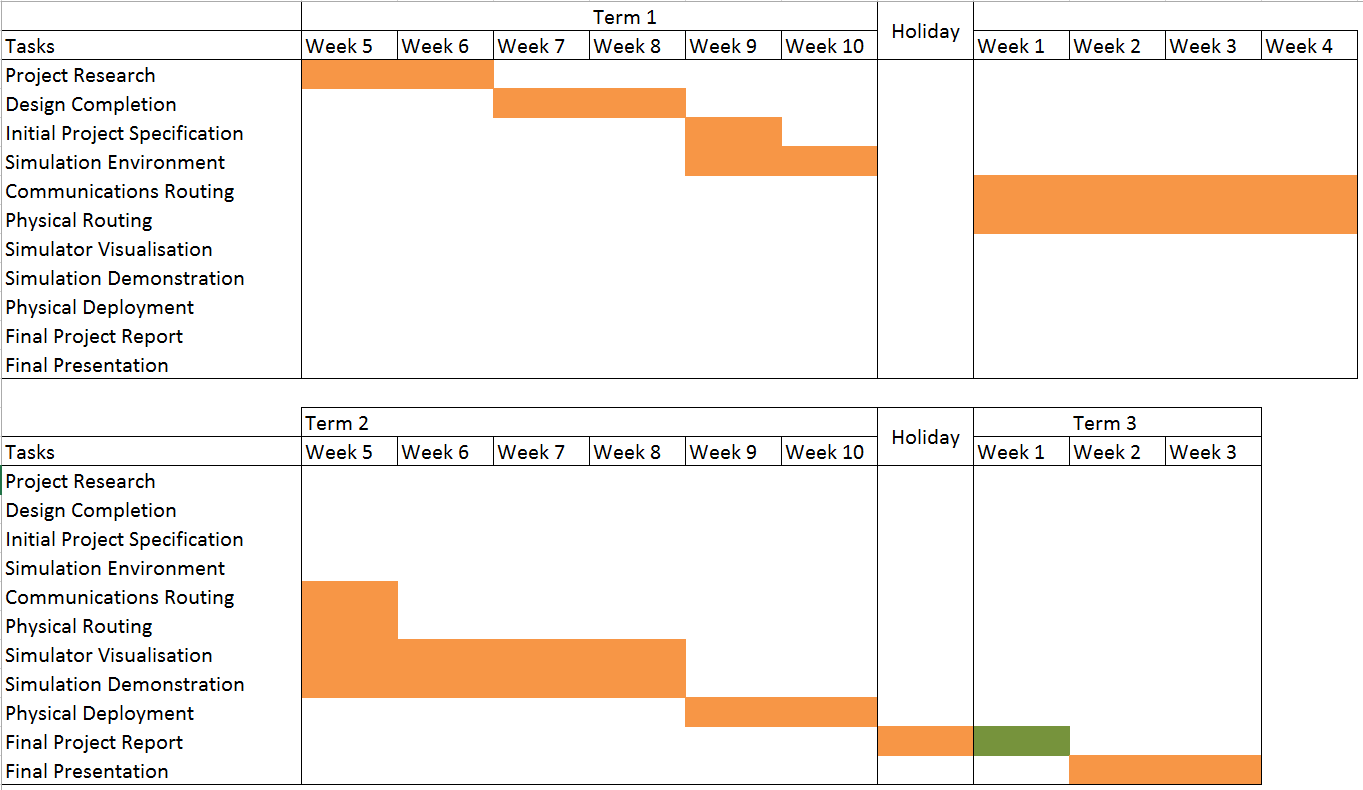
\includegraphics[scale=0.75,angle=90]{img/progantt.png}
\caption{Gantt chart of project schedule}
\label{gantt}
\end{figure}

\section{Progress Tracking}

\subsection{Meetings}
Regular meetings were scheduled once a week with both the project group and the project supervisor. Meetings with the supervisor consisted of sharing current progress, including any successes and challenges, as well as to seek advice on specific topics of difficulty such as simulation tools, accurately modelling error and routing techniques. Queries were also directed to the supervisor by email outside of meetings where necessary, to handle urgent requests or to check deliverables. 

The general group meetings involved all four members of the group gathering at the Department to discuss progress, assign new tasks as a result of discussions with the supervisor, or re-assign current tasks to improve scheduling. The group also examined the structure of the code, discussed bug fixes and new iterations of code, and corroborated any research findings using collaboration tools, which will be explained in section \ref{colab}. Extra meetings were also scheduled outside of the usual schedule in order to prepare for deadlines, or to coordinate workflow in the event of a task being assigned to more than one member. Certain tasks, such as physical deployment, required members to gather in one location in order to observe and work with the drones in person.

\subsection{Weekly Review}
In accordance with the software methodology chosen for the project, the group also informally discussed the status of the project in accordance with the schedule shown in figure \ref{timeline}, and received an update from each member as to their individual progress. By sharing the current state of each task with other members, it was possible to gauge the overall status of the project and to reassess any tasks which took up an inordinate amount of time. Instances of project review were also reserved for upcoming deadlines to ensure that project deliverables in particular were proceeding as planned. Minutes of meetings were kept in order to keep track of ongoing tasks.

\section{Source Control}
As a software-based project, it is important to ensure proper source control, so that code can be protected and members can be notified of new iterations, and how they differ from previous versions. While the source code itself did not have version numbers explicitly appended to it, Version Control Systems (VCS) were embedded into the collaboration tool used for code, including the ability to add messages which addressed the changes introduced by updated code, and to highlight any potential errors or bug fixes.

\section{Collaboration Tools}
\label{colab}

\subsection{GitHub}
To manage the project material, a git repository was created to ensure consistency amongst the project members' work and safety for the code base. Github, a web-based git repository hosting service, was used to incorporate source code management and distributed revision control to the project code. Each group member had their own repository locally, and branches were also used to ensure that major changes to the code base did not affect the original version of the code. This also allowed each member to avoid overwriting work when committing changes in the same area of code, which would result in merge conflicts. Using Github, the workflow was separated safely and manageably, and previous versions were retained by the repository so that they could not be lost. This also allowed each member of the group to contribute to the same repository without requiring them to be in the same physical space, or constantly exchanging updated code.

\subsection{Google Drive}
Google Drive was also used in order to manage project material, as well as have a backup for the code base and documentation. This is especially useful for project deliverables such as the report and the specification, as each member could collaborate in real-time with one another on the same documents. Google Drive also allowed for access on multiple devices such as phones, tablets and laptops, which was especially convenient for group meetings.

\subsection{Hastebin}
During the development of the project software, Hastebin was occasionally used for individual code snippets, as the UI supports code highlighting and is designed for sharing programming code. Alternatively, a real-time format such as Etherpad could have been used, but Hastebin was chosen for its ease-of-use and due to the fact that individual group members typically worked on separate areas of the same code, so Hastebin was utilised more for checking (incorrect) code than to develop code side-by-side.

\subsection{Facebook}
In order to communicate with other group members, Facebook was used as the primary method of contact. Each group member was already using Facebook, which made it the most common and the easiest way for group members to communicate. Facebook also allows for sharing files, which was found to be more convenient in the case of small files which did not require to be backed up. Facebook became a useful tool for general discussion about the project, including the project schedule and the code, as well as for the dissemination of tasks on-the-fly.

\section{Project Challenges}
At the beginning of the chapter, a summary was given of the main elements which the project was comprised of. In this section, the various challenges which had to be overcome in order to complete the project successfully are analysed. Specifically, areas such as researching, scheduling, organisation and development will be discussed, and how these challenges were dealt with throughout the project. 

\subsection{Planning}
The project was incredibly difficult in terms of the amount of work that had to be done in the limited amount of time available, and so effectively planning how and when each stage of the project would be completed was crucial to the project success. Each task which had to be completed was scheduled using the Gantt chart shown in figure \ref{gantt}, and the group was organised such that each member was aware of their individual tasks and responsibilities, and the timeframe available to them. The Gantt chart provided a good overview of the project activities, as well as being simple to read and understand; it was immediately clear that each member of the group what the current status of the project was, and what had to be completed at what time.

\subsection{Research}
One of the biggest challenges during the project was researching in order to find the proper tools and resources which were available that would be relevant to the project. A comparison of the various simulator libraries which were available was made, in order to find out their complexity, utilisation and functionality, such as ns-3 and OMNet++, and whether or not these libraries were necessary in order to create a drone sensor network. Ultimately, an original simulation was designed and developed by the group, which was influenced by the utilities provided by such libraries, and the use of ns-3 in the early stages of development was helpful to understand the various protocols which would need to be implemented into our own simulator.

\subsection{Development}
Following the planning stages, the project had carefully been broken down into tasks which had to be completed. According to the plan, the simulation would form the basis of physical deployment, in order to simplify the project as a whole and save time. During the development stage, the utmost care had to be taken to ensure that the simulation framework could be effectively transferred over to physical deployment during development. With this in mind, the simulation code was written in such a way that the only remaining factor to consider for physical deployment was the ability to use libraries which would interact with the drone's hardware, such as the ability to takeoff, move, turn, and land. Additionally, creating a simulation which could accurately model real-world communications without the use of network simulator libraries turned out to be a much more difficult task than had originally been scheduled for. The workload was subsequently re-evaluated and scheduled to realistically reflect the amount of time which would be taken, which involved using the time buffer of working over the holidays.

\subsection{Deployment}
When planning for physical deployment, there were several difficulties in terms of working with hardware which was not guaranteed to be suitable for the task. In order to provide autonomy to the drones, it was necessary to attach a Raspberry Pi to the drone, as well as GPS sensors, and then transfer the code base to the Pi in order to control the drone directly. Having no prior experience working with hardware explicitly, the group had to manage to configure the Pi in order to be able to connect and hook into the drone directly through Wi-Fi, and execute the code from the host (or base station). There were also concerns that attaching extra peripherals to the drone would potentially have weighed it down to the point that it would be incapable of sustaining its altitude, which would also affect its autonomous flight plan. The capabilities of the Parrot AR drone in terms of handling heavier payloads had to be researched and tested to confirm the maximum payload weight that it could handle.

\section{Risk Management}
The risks involved with the project are detailed in table \ref{risktable}.

\begin{table}
\centering
\caption{List of risks for the project}
\label{risktable}
\begin{tabular}{|p{0.5cm}|p{4.5cm}|p{8.5cm}|}
\hline
\# & Risk Event                                                           & Mitigation                                                                                                                                                               \\ \hline
1  & Team member falls ill during the project                             & Reassign tasks where necessary and focus on schedule. Use buffer time if necessary.                                          \\ \hline
2  & Parrot drones have faulty hardware                                   & Reason with Department for replacement hardware and focus on other tasks.                                                   \\ \hline
3  & Any hardware breaks or is faulty                                     & Same as 2 - replace where necessary or continue without if possible.                                                                                                     \\ \hline
4  & Lack of contribution from a team member                              & Attempt to encourage the team member and assist with the task if necessary. If problem persists, consult project supervisor. \\ \hline
5  & Development turns out to be too difficult technically                & Consult project supervisor for advice as to changing the project/project task/how to complete the task in question.          \\ \hline
6  & Code becomes corrupted or lost due to accident/damage                & Recover backup code from git repository and continue.                                                                                                                    \\ \hline
7  & Simulation environment is too slow to perform as needed              & Consider optimisation of simulation as priority over other tasks in order to preserve core functionality                     \\ \hline
8  & Research for drone sensor networks is limited                        & Focus on combinations of alternatives e.g. research on drones, research on sensor networks                                  \\ \hline
9  & Unable to implement visualisation for the simulation                 & Focus on ensuring that other key functionality is achieved/maintained for the simulator and consider as future work          \\ \hline
10 & Drone gets lost during deployment due to loss of signal/out of range & Liaise with campus security to arrange for retrieval of the drone                                                                                                                                                    \\ \hline
11 & Communications routing is too difficult/time costly to implement     & Consider finding and using pre-existing libraries which can be imported to the stimulator                                  \\ \hline
12 & Physical routing is too difficult/time costly to implement           & Consider reverting to core functionality or pre-existing libraries where necessary  
                                        \\ \hline
\end{tabular}
\end{table}

\begin{table}
\begin{tabular}{|p{0.5cm}|p{4.5cm}|p{8.5cm}|}
\hline
\# & Risk Event                                                           & Mitigation                                                                                                                                                               \\ \hline
13 & Drones are unable to perform collision detection                     & Ensure that drones manage individual, well-separated airspace only and are physically unable to go near each other           \\ \hline
14 & Physical deployment is not completed on time                         & Focus on functionality of the simulator for demo and present theoretical results for real deployment where possible         \\ \hline
15 & Scheduling is poorly managed and tasks are overestimated timewise    & Re-evaluate schedule and use buffer time if necessary. Tasks may also be added or removed where necessary                    \\ \hline
16 & Demonstration code for simulation is not completed on time           & Revert to using example code used to test simulation for demo and physical deployment.                                      \\ \hline
17 & Use of drones on campus is deemed illegal/unsanctioned               & Find open airspace in alternate location which is not monitored/free to use                                             \\ \hline
\end{tabular}
\end{table}

\section{Legal, Social, Ethical, and Professional Issues}
The subject of drones has been the focus of much controversy with regards to issues of privacy, invasion of airspace and other unsanctioned uses of UAVs with the ability to, for example, use a camera to take pictures or video. Therefore, a platform for an entire network of drones with a variety of sensors which is open source presents a multitude of possible problems. Furthermore, with the potential to be used as a foundation for military efforts, which form the basis of many current topics of research into drones and sensor networks, there are many implications for potential misuse of the project. As a result, it is necessary to research and discuss the possible methods of unlawful utilisation of drones and drone networks, in order to ensure that the project group is aware of these issues.

\subsection{Legal Issues}
The law is, however, very clear with regards to the use of firearms against UAVs, whether or not the UAV in question was trespassing or invading on private property. In November 2014, a man was fined \$850 in damages for shooting down a neighbour’s drone while it was flying over the neighbour's property, and then refusing to pay any compensation for destroying the drone \cite{colinneagle2015}. The Federal Aviation Administration’s (FAA) definition of a drone as aircraft also means that, technically, shooting a drone could result in a maximum penalty of a 20 year prison sentence. Pursuing legal action in cases such as this is difficult, as it is not illegal to fly a drone in public. 

There are several instances where the definition of misuse of drones has been well established and offenders have been prosecuted. In the very first case of prosecution against unsanctioned drone usage, a security guard was sentenced after repeatedly flying drones over and around Premier league football stadiums, Buckingham Palace and Parliament buildings, where he was fined and banned from flying UAVs \cite{maryannrusson2015}.  In the US, FAA regulations state that drones must not be flown near airports and other areas with manned aircraft, as well as placing a ban on altitudes over 400ft. The Civil Aviation Authority (CAA) in the UK states that for a Small Unmanned Surveillance Aircraft (SUAS) of less than 20 kg, the operation must not endanger anyone or anything, and the aircraft must be within visual line of sight \cite{civilaviationauthority2015}.

For the specific case outlined above, the aircraft being used for surveillance purposes was in violation of the rules of direct line of sight of the aircraft as well as being subjected to tighter restrictions with regard to the minimum distances that you can fly near people or properties that are not authorised. In most instances of prosecution, the owner of the drone would be required to have permission from the CAA to fly their drone in an area that would usually be forbidden access.

There have also been cases of the use of drones in order to smuggle illegal substances into high security areas. Scotland Yard has logged various different drone-related incidents, including complaints about drones being used to ferry drugs into prison \cite{maryannrusson2015}.  It is highly likely that an individual or individuals would be responsible for such use of drones, particularly in violation of multiple laws \cite{civilaviationauthority2015}, as opposed to commercial businesses. However, this implies that open source autopilot software and other similar platforms may be used unlawfully by individuals.

\subsection{Social Issues}
A interesting issue arises where any drone carrying a payload such as a camera has the potential for recording data unlawfully. In one instance, a drone which was found to be hovering over an ATM that seemed to be recording people entering their pin numbers into a cash machine. It can be argued that the drone was not breaking the law by simply recording a public space\cite{maryannrusson2015}. However, it is difficult to prove that the usage of the drone was for the express purpose of obtaining peoples’ pin number, or if this is unlawful to begin with, in the same way that there is no law which expressly forbids someone from looking over the shoulder of an ATM user.

A full-length documentary called Speciesism: The Movie based its foundational discoveries and source of information by using drones to spy on factory farms and record evidence of environmental damage, and went on to feature major global press coverage. In this particular instance, the law with regards to prosecution was unclear, despite the activity being labelled as ‘spying’. This could suggest that such uses of drones, even on potentially private property, may not be possible to prosecute, although this may be unique to incidences of whistleblowing. It will be up to society to determine where the acceptable boundaries of drone usage lie, and how this should be represented in legislation.

\subsection{Ethical Issues}
As discussed in previous sections, engaging in military operations is one of the most prevalent uses for drones, as well as being a popular area for research and development of UAVs. Fortunately, the specifications of consumer-level drones are not of a high enough calibre to warrant usage in the military, which requires state-of-the-art hardware, including weaponry. However, there is an initiative to create small, hand-sized mini drones for soldiers in the US Army, for the purpose of small scale intelligence gathering and reconnaissance, in place of conventional air support \cite{jonfingas2016}. Projects such as this have implications for the usage of drones of all shapes and sizes in military operations, which would suggest that implementations of drone autonomy by hobbyists and businesses may form a basis for research and development in the army.

The use of drones for spying is not only limited to consumers, militaries have also been responsible for deploying drones to spy on civilians in their home country. The Department of Defense in the United States has admitted to using Predator and Reaper military drones in the US since 2006 in order to support domestic civil authorities, which was made public in March 2016 \cite{pentagon2016}. According to the government, these domestic drone flights are stated as not being in violation of any laws, and were being employed in a “very, very minimal way, very seldom”.

\subsection{Professional Issues}
Given that the project is released under an open source license, it is possible that it will be used to perpetrate acts which are illegal or unethical. If there should be an onus on creators to restrict the functionality of their projects, then this has troubling implications in terms of free speech. Additionally, there are many use cases of drones which could be classified as either ethical or unethical depending on intent (reconnaissance for a police drugs raid compared to reconnaissance for a bank heist). 
